\documentclass[pdftex,12pt,letter]{article}
\usepackage{fancyhdr}
\usepackage{enumerate}
\usepackage{tabularx}
\usepackage{graphicx}
\usepackage{array}
\usepackage{hyperref}
\usepackage[justification=justified,singlelinecheck=false]{caption}
\usepackage{placeins}
\usepackage{rotating}
\makeatletter
  \renewcommand\@seccntformat[1]{\csname the#1\endcsname.\quad}
\makeatother

\newcolumntype {Y}{ >{\raggedright \arraybackslash }X}
\newcommand{\HRule}{\rule{\linewidth}{0.5mm}}
\captionsetup{labelformat=empty}

\begin{document}

\begin{titlepage}
\begin{flushright}
\HRule \\[0.4cm]
{ \bfseries
{\huge CWRUtility Bug Reports\\[1cm]}
{\Large for\\[1cm]}
{\huge CWRUtility\large\\[4cm]}
{\large Prepared by\\Stuart Long\\[1cm]
Version 1.2\\[1cm]
KOALAA Development\\[1cm]
December 7, 2012}}
\end{flushright}
\end{titlepage}
\begin{table}[!t]
\caption*{\bfseries Revision History}
\begin{tabularx}{\textwidth }[t]{|l|Y|Y|l|}
\hline
\bfseries Name & \bfseries Date & \bfseries Reasons for Change & \bfseries Version \\ \hline
Long & 12/6/2012 & Initial Draft & 1.0\\
\hline
\end{tabularx}
\end{table}
\FloatBarrier
\newpage
\clearpage
\section{Introduction}
The CWRUtility development team uses an online software suite to log and track any bugs/feature requests/maintenance issues in the application. Specifically, the suite used is 
\url{http://www.fogcreek.com/fogbugz/}. Since only the development team has access to the CWRUtility project within the tracking system, screenshots of the current bug reports have been included below. 
\newpage
\begin{sidewaysfigure}
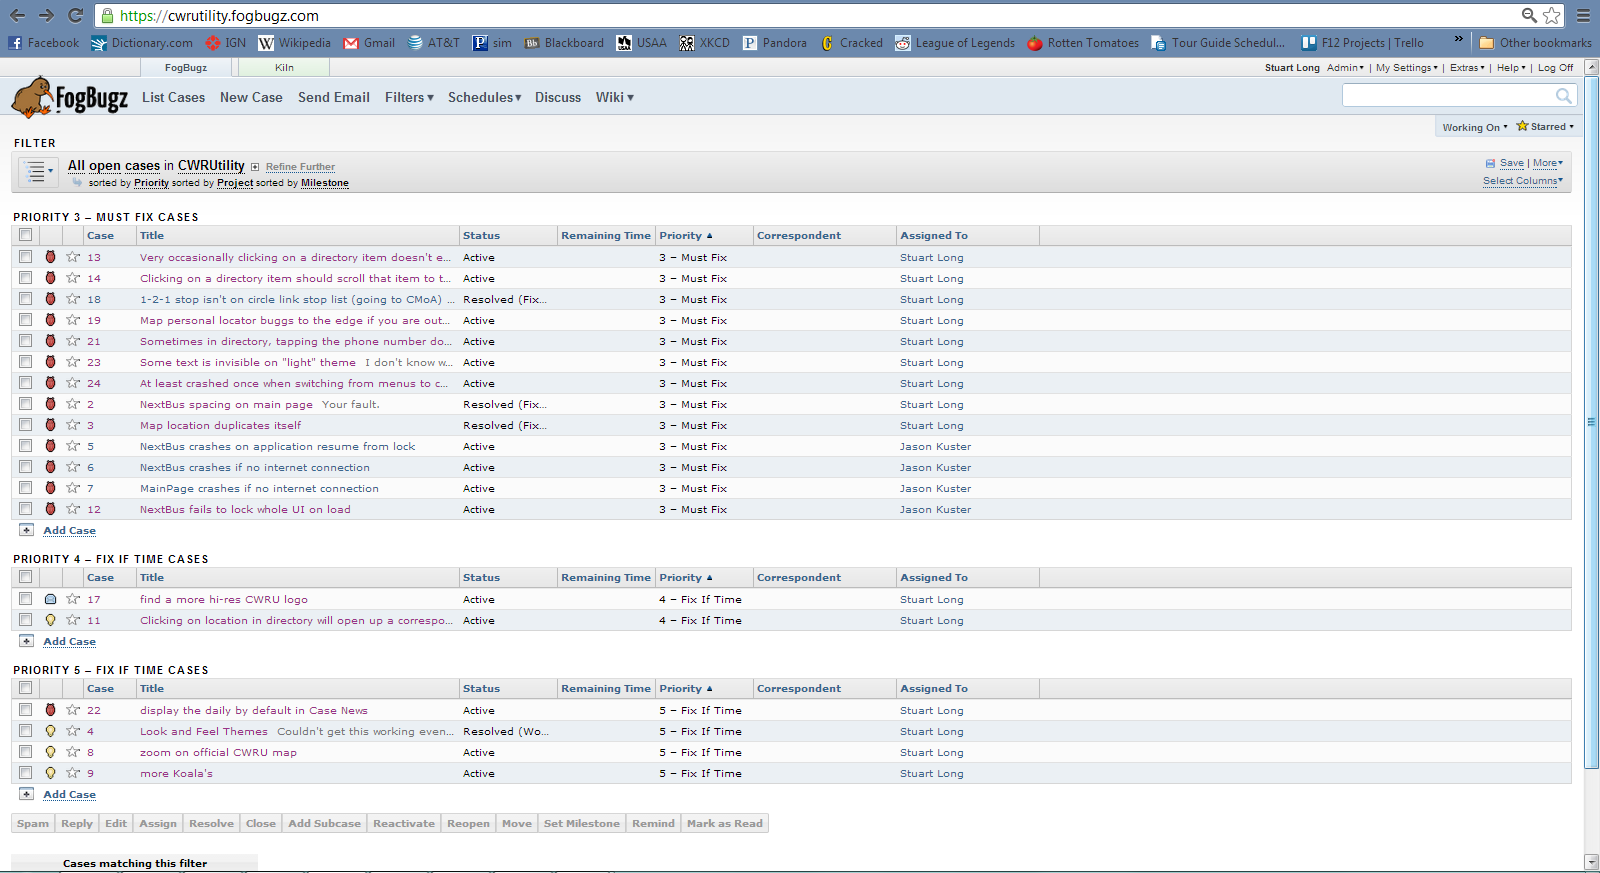
\includegraphics[width=9in]{bugs1.png}
\end{sidewaysfigure}
\FloatBarrier
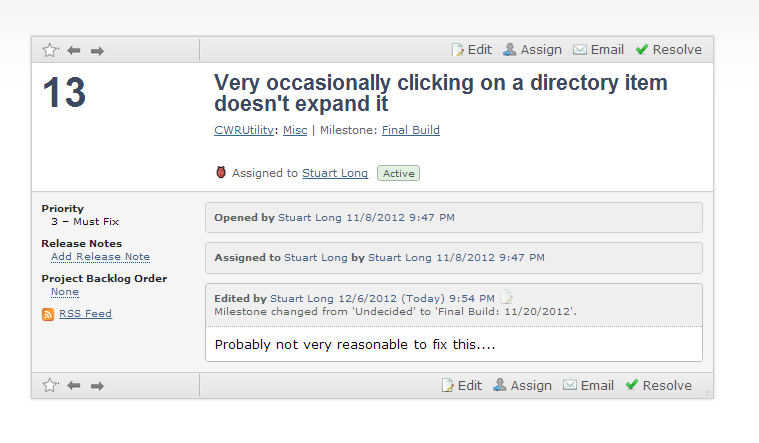
\includegraphics[width=4in]{bugs2.png}
\FloatBarrier
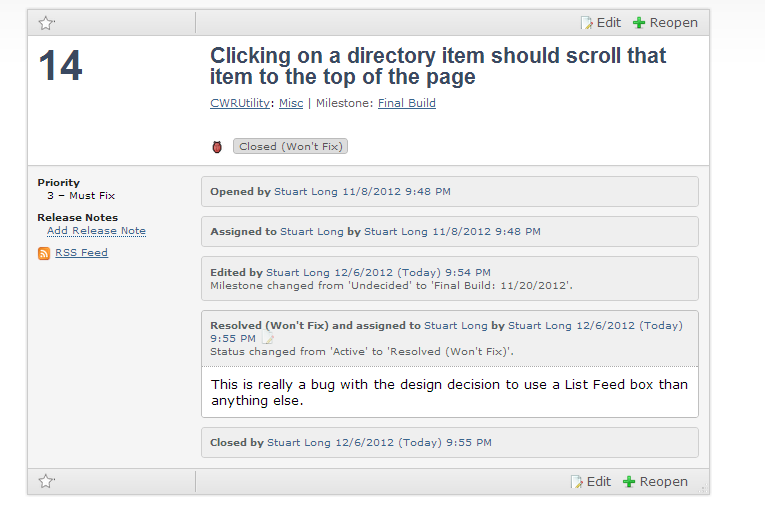
\includegraphics[width=4in]{bugs3.png}
\FloatBarrier
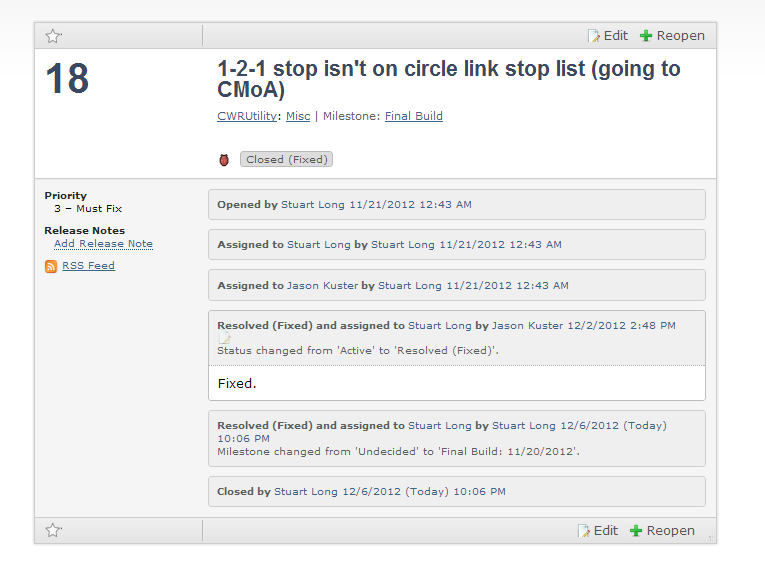
\includegraphics[width=4in]{bugs4.png}
\FloatBarrier
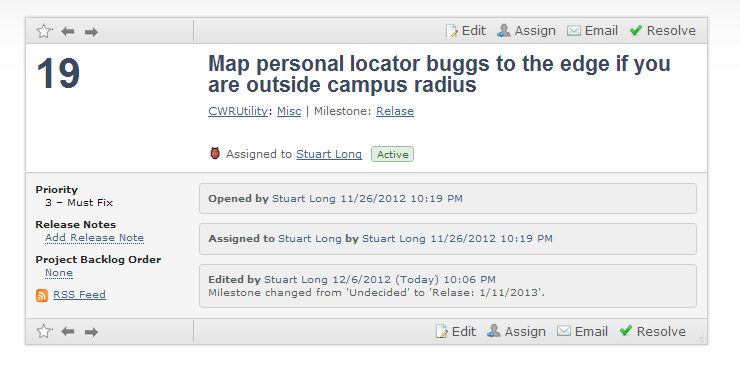
\includegraphics[width=4in]{bugs5.png}
\FloatBarrier
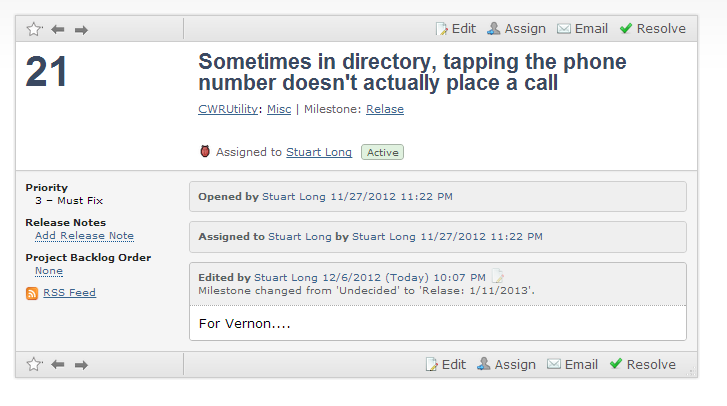
\includegraphics[width=4in]{bugs6.png}
\FloatBarrier
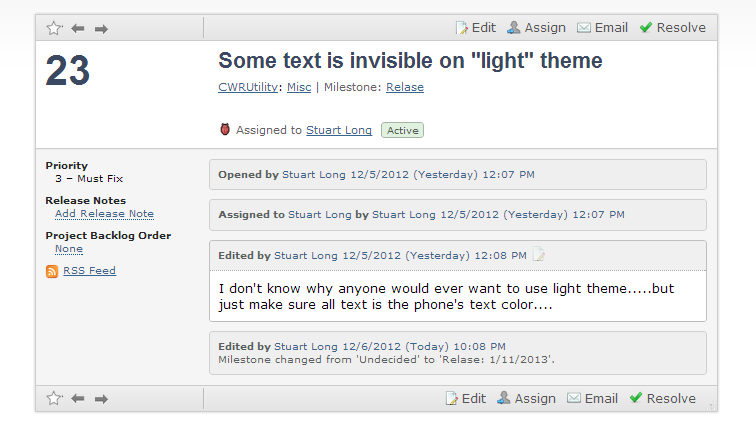
\includegraphics[width=4in]{bugs7.png}
\FloatBarrier
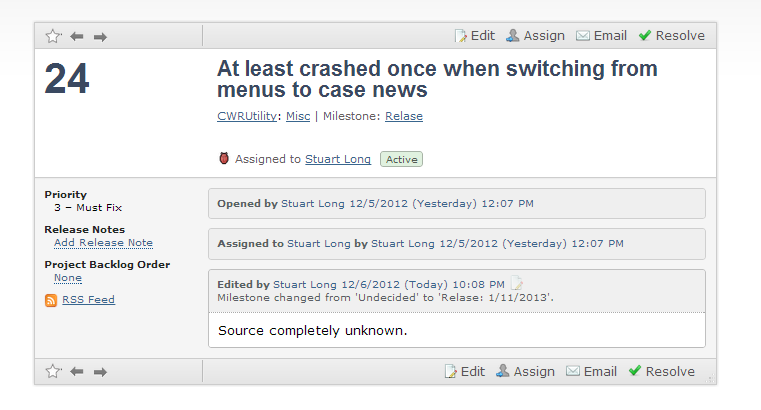
\includegraphics[width=4in]{bugs8.png}
\FloatBarrier
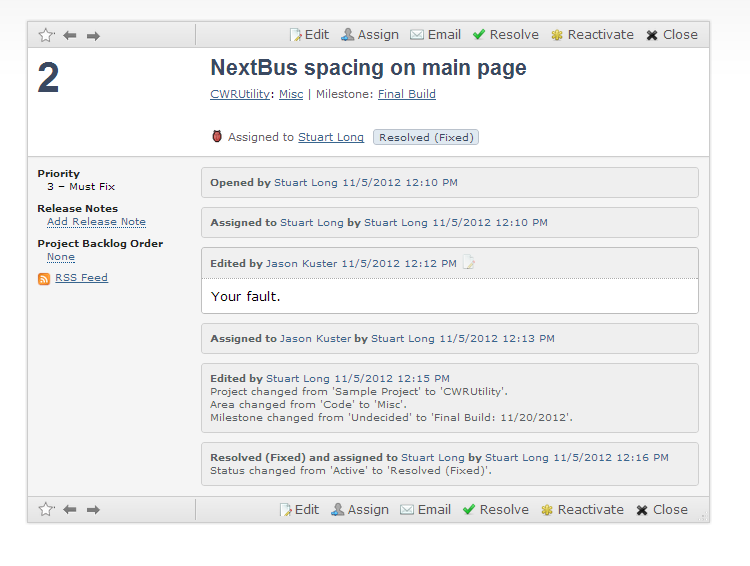
\includegraphics[width=4in]{bugs9.png}
\FloatBarrier
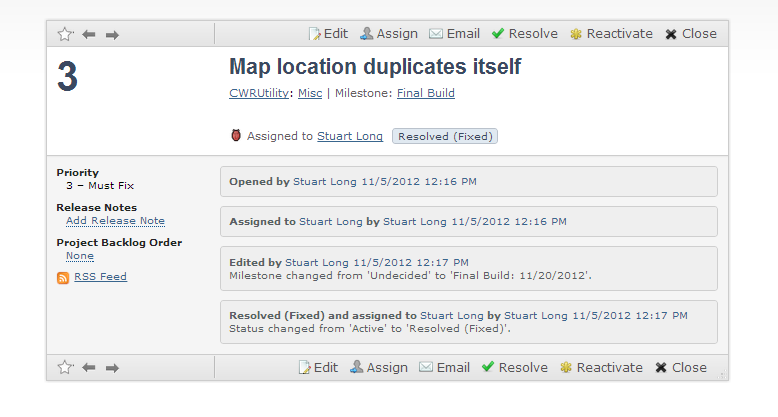
\includegraphics[width=4in]{bugs10.png}
\FloatBarrier
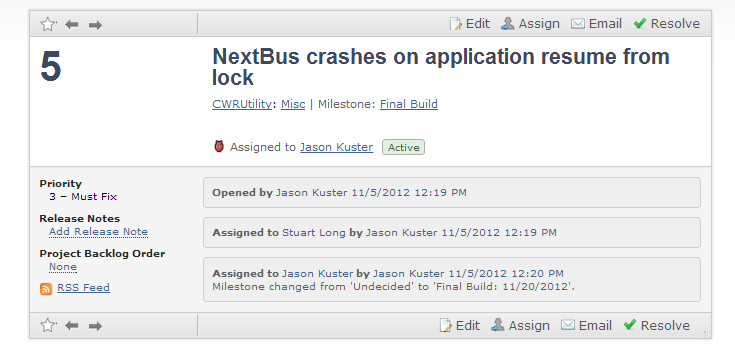
\includegraphics[width=4in]{bugs11.png}
\FloatBarrier
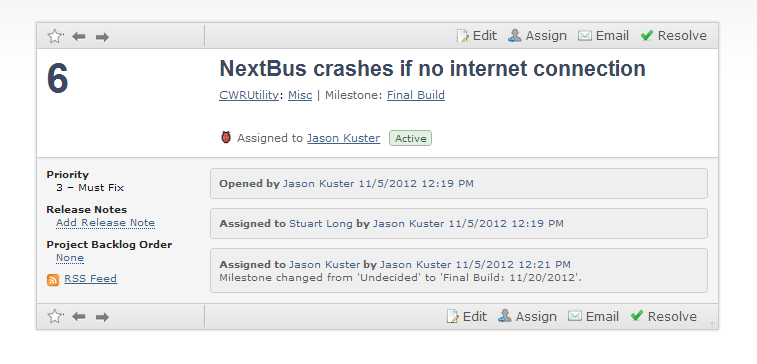
\includegraphics[width=4in]{bugs12.png}
\FloatBarrier
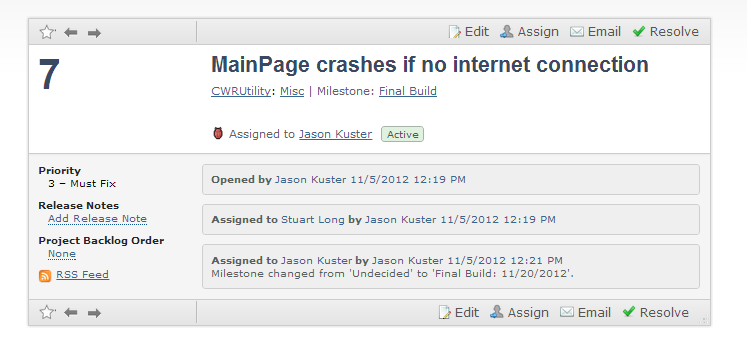
\includegraphics[width=4in]{bugs13.png}
\FloatBarrier
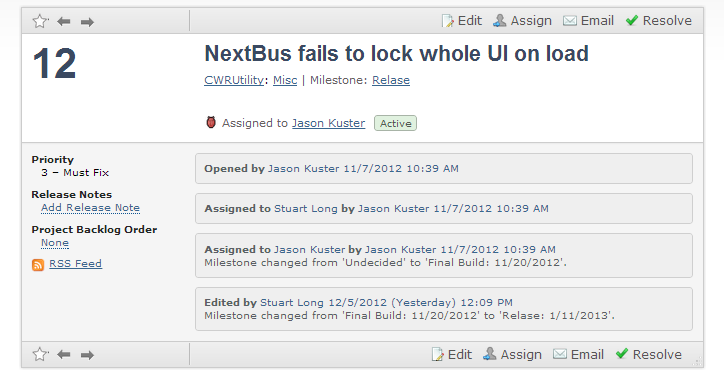
\includegraphics[width=4in]{bugs14.png}
\FloatBarrier
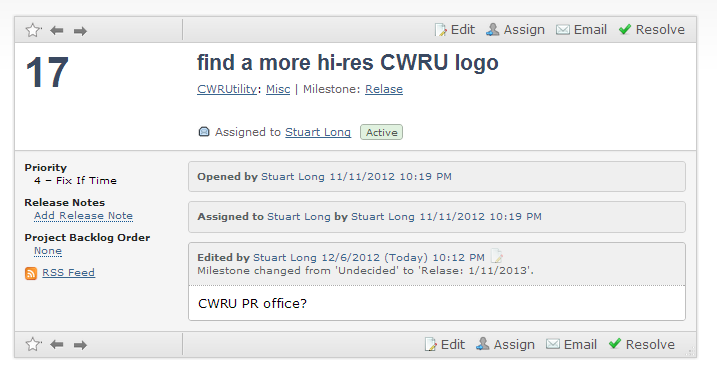
\includegraphics[width=4in]{bugs15.png}
\FloatBarrier
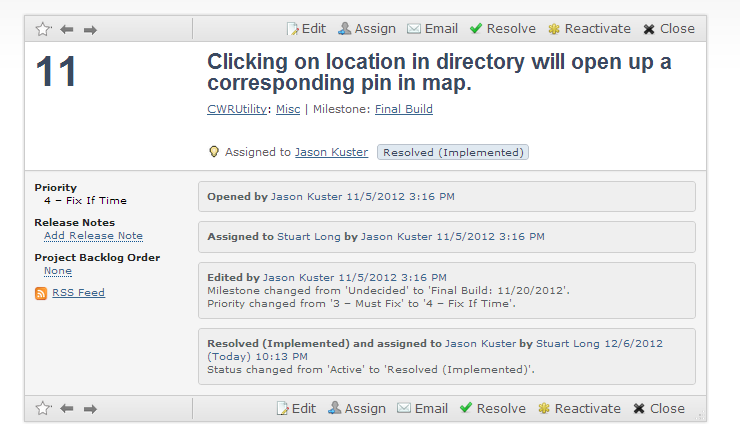
\includegraphics[width=4in]{bugs16.png}
\FloatBarrier
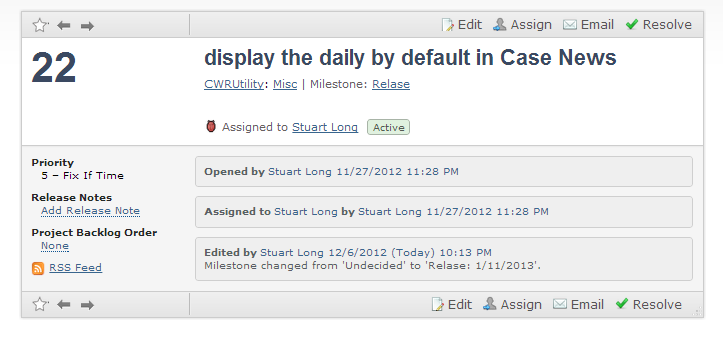
\includegraphics[width=4in]{bugs17.png}
\FloatBarrier
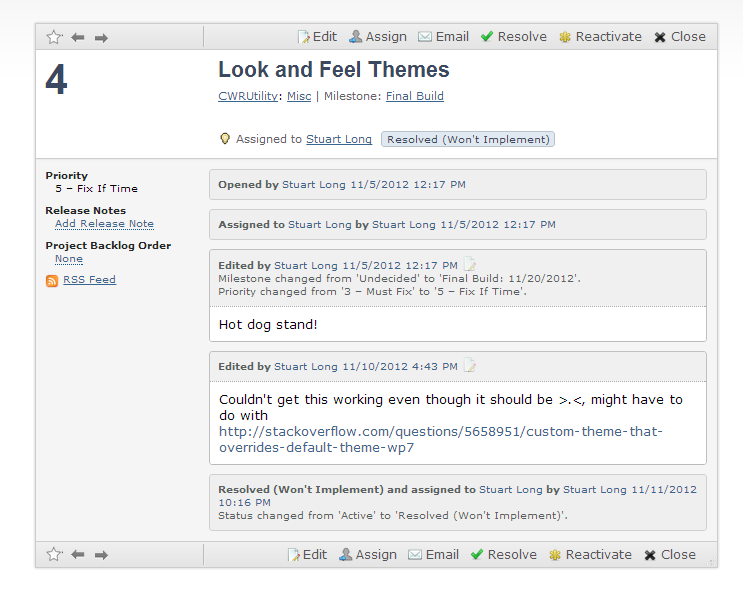
\includegraphics[width=4in]{bugs18.png}
\FloatBarrier
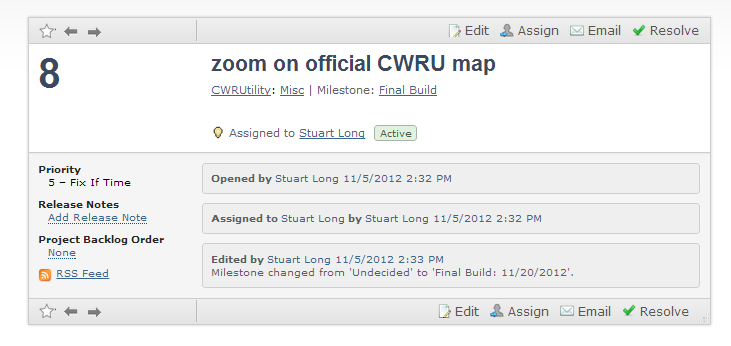
\includegraphics[width=4in]{bugs19.png}
\FloatBarrier
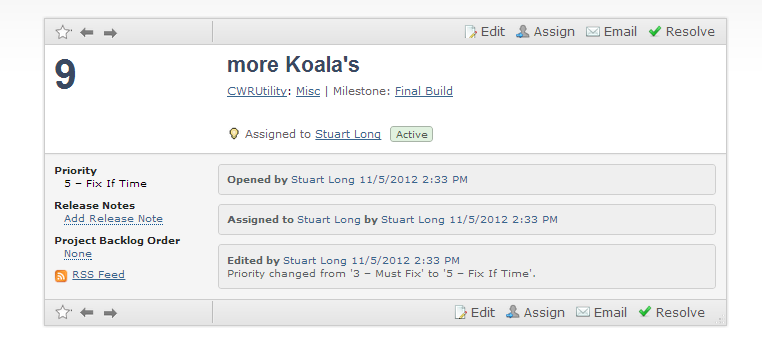
\includegraphics[width=4in]{bugs20.png}
\FloatBarrier
\lfoot{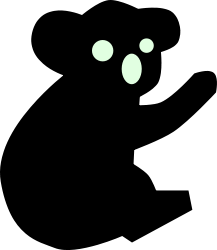
\includegraphics[height=1cm]{DarkKoala.png}}
\end{document}